\documentclass[a4paper]{article}

\usepackage{inputenc}
\usepackage[british,UKenglish]{babel}
\usepackage{amsmath}
%\usepackage{titlesec}
\usepackage{color}
\usepackage{graphicx}
\usepackage{fancyref}
\usepackage{hyperref}
\usepackage{float}
\usepackage{scrextend}
\usepackage{setspace}
\usepackage{xargs}
\usepackage{multicol}
\usepackage{nameref}

\usepackage{sectsty}
\usepackage{multicol}
\usepackage{multirow}
\usepackage[procnames]{listings}
\usepackage{appendix}
\usepackage{listings}

\newcommand\tab[1][1cm]{\hspace*{#1}}
\hypersetup{colorlinks=true, linkcolor=black}
\interfootnotelinepenalty=10000

\newcommand{\cleancode}[1]{\begin{addmargin}[3em]{3em}\texttt{\textcolor{cleanOrange}{#1}}\end{addmargin}}
\newcommand{\cleanstyle}[1]{\text{\textcolor{cleanOrange}{\texttt{#1}}}}


\usepackage[colorinlistoftodos,prependcaption,textsize=footnotesize]{todonotes}
\newcommandx{\commred}[2][1=]{\textcolor{Red}
{\todo[linecolor=red,backgroundcolor=red!25,bordercolor=red,#1]{#2}}}
\newcommandx{\commblue}[2][1=]{\textcolor{Blue}
{\todo[linecolor=blue,backgroundcolor=blue!25,bordercolor=blue,#1]{#2}}}
\newcommandx{\commgreen}[2][1=]{\textcolor{OliveGreen}{\todo[linecolor=OliveGreen,backgroundcolor=OliveGreen!25,bordercolor=OliveGreen,#1]{#2}}}
\newcommandx{\commpurp}[2][1=]{\textcolor{Plum}{\todo[linecolor=Plum,backgroundcolor=Plum!25,bordercolor=Plum,#1]{#2}}}

\def\code#1{{\tt #1}}

\def\note#1{\noindent{\bf [Note: #1]}}

\makeatletter
%% The "\@seccntformat" command is an auxiliary command
%% (see pp. 26f. of 'The LaTeX Companion,' 2nd. ed.)
\def\@seccntformat#1{\@ifundefined{#1@cntformat}%
   {\csname the#1\endcsname\quad}  % default
   {\csname #1@cntformat\endcsname}% enable individual control
}
\let\oldappendix\appendix %% save current definition of \appendix
\renewcommand\appendix{%
    \oldappendix
    \newcommand{\section@cntformat}{\appendixname~\thesection\quad}
}
\makeatother




\lstset{frame=, basicstyle={\footnotesize\ttfamily}}



\graphicspath{ {images/} }
\usepackage{ctex}
%-----------------------------------------BEGIN DOC----------------------------------------

\begin{document}
\renewcommand{\contentsname}{目\ 录}
\renewcommand{\appendixname}{附录}
\renewcommand{\appendixpagename}{附录}
\renewcommand{\refname}{参考文献} 
\renewcommand{\figurename}{图}
\renewcommand{\tablename}{表}
\renewcommand{\today}{\number\year 年 \number\month 月 \number\day 日}

\title{{\Huge CS22014实验报告模版{\large\linebreak\\}}{\Large 实验二、GPU PTX与线程管理\linebreak\linebreak}}
%please write your name, Student #, and Class # in Authors, student ID, and class # respectively
\author{\\姓\ 名:计\ 春\ 生\\
学\ 号: 168668\\
班\ 号: xxxxx\\\\
CS 22014 流计算结构及其程序设计\\
(春季, 2017)\\\\
西北工业大学\\
计算机学院\\
ERCESI}
\date{\today}
\maketitle
\newpage

%-----------------------------------------ABSTRACT-------------------------------------
\begin{center}
{\Large\bf{摘\ 要\\}}
\end{center}
请在这里输入摘要内容.
\newpage
%-----------------------------------------ABSTRACT-------------------------------------
\begin{center}
{\Large\bf{版\ 权\ 声\ 明\\}}
\end{center}
该文件受《中华人名共和国著作权法》的保护。ERCESI实验室保留拒绝授权违法复制该文件的权利。任何收存和保管本文件各种版本的单位和个人,未经ERCESI实验室(西北工业大学)同意,不得将本文档转借他人,亦不得随意复制、抄录、拍照或以任何方式传播。 否则,引起有碍著作权之问题,将可能承担法律责任。\newpage
%-----------------------------------------CONTENT-------------------------------------
\begin{center}
\tableofcontents\label{c}
\end{center}
\newpage

%------------------------------------------TEXT--------------------------------------------

%----------------------------------------OVERVIEW-----------------------------------------

\section{概述} \label{overview}%------------------------------
这一节请主要描述这次实验的主要实验内容。由于latex的中文使用了ctex包,所以需要xelatex进行编译。
\begin{itemize}
	\item{\textbf{PTX分析} 分析NVidia GPGPU PTX指令,判断实现矩阵运算需要的指令序列}
    \item{\textbf{与x86指令进行比较} 比较GPGPU指令序列和x86标量指令序列实现矩阵运算的差异}
    \item{\textbf{分析Warp调度的过程} 寻找GPGPU-sim中关于Warp调度管理的代码,分析计分牌算法}
    \item{\textbf{warp调度的实验} 分析不同的指令序列的warp调度能力,分别设定能够掩盖存储延时和不能掩盖存储访问延时的不同序列,分析计算性能。}
\end{itemize}

%------------------------------------Lab Process--------------------------------------

\newpage
%------------------------------
\section{PTX指令序列产生}\label{sub:ptx}
\subsection{实验过程} \label{sub:ptxproc}
建议使用listings package来表示不同显示不同的命令行或代码。使用如下代码:
\begin{lstlisting}[language=bash]
$source setup release
\end{lstlisting}
如果使用图进行说明,Latex中插入图并进行索引的方式如下:图\ref{fig:singleblock}. 
\begin{figure}[ht]
 \centering
 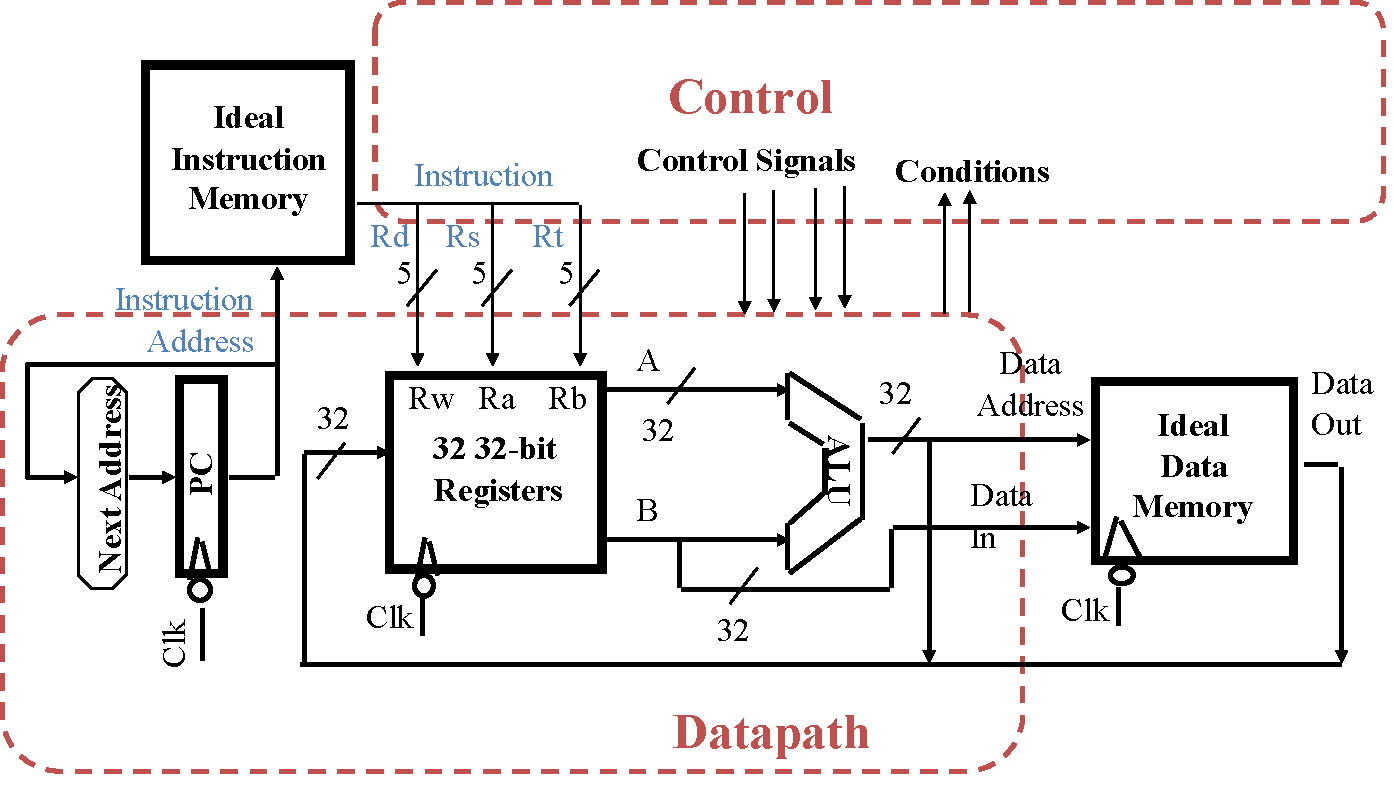
\includegraphics[height=5cm]{images/l1sys.pdf}
 \caption{单周期处理器结构图}
 \label{fig:singleblock}
\end{figure}
如果需要索引参考文献,请使用\cite{Erdos01}, 同时已经将参考文献的项目模版在文末写出。

如果需要表格,可以建立类似表\ref{tab:signaldef}这样的列表进行说明。

\begin{table}[htp]
\caption{测试模式信号定义}\label{tab:signaldef}
\begin{center}
	\begin{tabular}{|l|l|l|p{6cm}|}
	\hline
	\textbf{信号名} & \textbf{方向} & \textbf{位宽} & \textbf{功能描述}\\ \hline \hline
	boot			& Input 	& 1-bit	& 触发测试模式, 当处理器正常工作时被置为0\\ \hline
	test\_im\_wr 	& Input	& 1-bit	& Instruction memory write enable in test mode,set to 0 in 	
								  CPU regular process mode. In test mode, it will be set to 1 when if writing instructions to imem, otherwise it is set to 0.\\ \hline
	test\_im\_re 	& Input & 1-bit & Instruction memory read enable in test mode,set to 0 in 	
								  CPU regular process mode. In test mode, it will be set to 1 when if reading instructions out, otherwise it is set to 0. \\ \hline
	test\_im\_addr 	& Input & 32-bit& Instruction memory address\\ \hline
	test\_im\_in 	& Input & 32-bit& Instruction memory data input for test mode. \\ \hline
	test\_im\_out 	& Output& 32-bit& Instruction memory data output for test mode. \\ \hline
	test\_dm\_wr 	& Input	& 1-bit	& Data memory write enable in test mode,set to 0 in 	
								  CPU regular process mode. In test mode, it will be set to 1 when if writing data to dmem, otherwise it is set to 0.\\ \hline
	test\_dm\_re 	& Input & 1-bit & Data memory read enable in test mode,set to 0 in 	
								  CPU regular process mode. In test mode, it will be set to 1 when if reading data out, otherwise it is set to 0.\\ \hline
	test\_dm\_addr 	& Input & 32-bit& Data memory address\\ \hline
	test\_dm\_in 	& Input & 32-bit& Data memory input for test mode. \\ \hline
	test\_dm\_out 	& Output& 32-bit& Data memory output for test mode. \\ \hline
	valid			& Output& 1-bit & If CPU stopped or any exception happens, valid signal is set to 0.\\ 
	\hline
	\end{tabular}
\end{center}
\end{table}

\subsection{实验结果和分析}\label{sub:ptxeva}
请在这一节详细说明需要分析的内容。
% --------------------------------Evaluation----------------------------------------
\section{PTX与x86指令的比较}\label{ptxvsx86}
以下请按照上面的说明示例,自行安排章节内容。

% -----------------------------------Appendix----------------------------------------
\appendix
\section{代码}\label{sub:app.code}
请在附录\ref{sub:app.code}中添加代码。请使用如下C或者C++的语法高亮描述方法。
\begin{lstlisting}[language=C]
class TopIO extends Bundle() {
	val boot = Input(Bool()) 
// imem and dmem interface for Tests
	val test_im_wr		= Input(Bool())
	val test_im_rd 		= Input(Bool())
	val test_im_addr 	= Input(UInt(32.W))
	val test_im_in 		= Input(UInt(32.W))
	val test_im_out 	= Output(UInt(32.W))

	val test_dm_wr		= Input(Bool())
	val test_dm_rd 		= Input(Bool())
	val test_dm_addr 	= Input(UInt(32.W))
	val test_dm_in 		= Input(UInt(32.W))
	val test_dm_out 	= Output(UInt(32.W))

	val valid			= Output(Bool())
}
class Top extends Module() {
	val io 		= IO(new TopIO())//in chisel3, io must be wrapped in IO(...) 
	//...
	when (io.boot & io.test_im_wr){
		imm(io.test_im_addr) := io.test_im_in
		} .elsewhen (io.boot & io.test_dm_wr){
		// please finish it
		} //...
}
\end{lstlisting}
\newpage
% -----------------------------------REFERENCE----------------------------------------
\begin{thebibliography}{9}
\bibitem{Erdos01} P. Erd\H os, \emph{A selection of problems and
results in combinatorics}, Recent trends in combinatorics (Matrahaza,
1995), Cambridge Univ. Press, Cambridge, 2001, pp. 1--6.
\end{thebibliography}
\end{document}

